\chapter{Multi Group Key Management Protocol}
\label{chap:mgkmp}

The main mission of the internship is to continue the underway research work on the Multi Group Key Management Protocol (MGKMP), being conducted within the host lab. Section~\ref{sec:mgkmp_overview} presents key elements the work done so far. It's kind of a literature review specific to the lab's scientific production. The rest of this chapter sums up the first assignment, which consists in the in-depth study of the protocol and identification of work yet to be done.

\section{Overview of MGKMP}
\label{sec:mgkmp_overview}

The MGKMP is organized in three layers. The first layer is intended for node and key management. Each node is assigned to a subgroup $S^i_j$ of the group $G_i$. Managed keys can be categorized into Data Encryption Keys (DEKs) and Key Encryption Keys (KEKs). These keys are either used for device-to-device communications (pairwise keys) or group and subgroup communications. The second layer is intended for subgroup management. This partitioning considerably decreases the nodes' storage overhead. The third and last layer is intended for service and group management. Groups are chosen according to a unique combination of services. Fig.~\ref{fig:mgkmp_layers} illustrates the MGKMP architecture. Still to note that subgroups layer is logical and totally transparent to the application layer.

\begin{figure}[htbp]
	\centerline{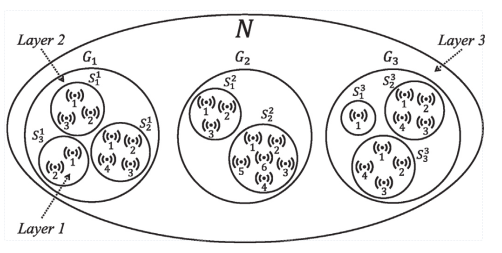
\includegraphics[scale=0.60]{figures/mgkmp/mgkmp_layers.png}}
	\caption{Source \cite{kandi_versatile_2020}: Example of a network partitioning}
	\label{fig:mgkmp_layers}
\end{figure}

The protocol aims at ensuring five different properties: scalability, efficiency, heterogeneity, collusion resistance and forward and backward secrecy. The two last properties are security oriented, whereas the first three ones are used to evaluate the protocol's performance. Forward secrecy is guaranteed when a leaving member of a group has no longer access to his former group communications. Backward secrecy is guaranteed when a joining member of a group has no access to his group's old communications. A collusion attack unfolds when multiple compromised nodes (evited or not) cooperate using their individual pieces of information to gain illegitimate access to the group key. To curb these security risks, the protocol relies on keys revokes and rekeying operations. Every time a node is joining, leaving or evicted from a group, all pairwise keys associated with these node as well as related group keys are revoked and new ones are generated. Rekeying operations and group memberships are handled by the Key Manager (KM). This makes the KM the protocol's security backbone.

Among key contributions of MGKMP is its compatibility with heterogeneous networks. Giving the increasingly sophisticated and inter-connected nature of IoT networks, this is a major asset.

\section{Optimization of MGKMP}
\label{sec:mgkmp_optimization}

These working tracks consider mainly the optimzsation of the MGKMP protocol. The idea consists in redesigning some aspects of the protocols features, and then comparing the new design’s complexity and other properties with the original design. Presumably, each optimization brought should be compared apart, and eventually, a combination of those could be tested. The ultimate objective is to produce a better optimized version of MGKMP in terms of security, resilience, flexibility, efficiency and scalability.

\subsection{Analysis of an n-tier architecture}
\label{subsec:n-tier}

The first subgroup layer in the paper aims at grouping devices by physical capacity and power. Thereby, it decreases energy drainage for devices. But this extra layer piles up complexity to the overall architecture and cryptographic key management, whether those used for group or device-to-device communications. This complexity increase shadows on the raising number of required messages during rekeying operations, and therefore, an increase in network traffic and bandwidth consumption. However, network traffic indulged on a network adapter is itself a factor of energy drainage for the device.

Now let’s imagine an extension of the suggested protocol to a 4-tier architecture. This might contribute to the enhancement of the storage overhead and computation effort for a device node. But it would probably lead to ever further utilization of network bandwidth as well, and so, the device battery might waste on network adapters what it had saved from its CPU. However, the study of both aspects of the protocol’s performance shall lead to a proper compromise.

\begin{figure}[htbp]
	\centerline{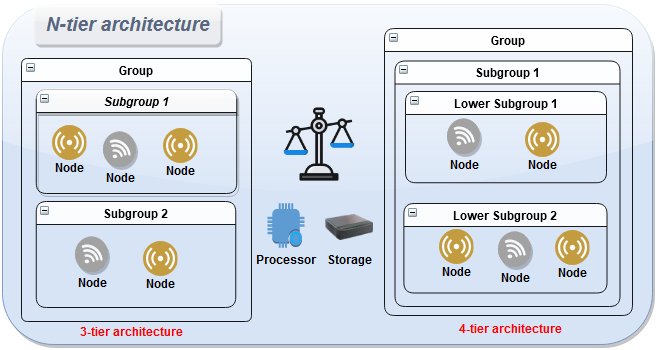
\includegraphics[scale=0.60]{figures/mgkmp/n-tier.png}}
	\caption{3-tier architecture vs. 4-tier architecture}
	\label{fig:n-tier}
\end{figure}

A naive question to sum up the issue would be:

\begin{quote}
	\emph{What consumes more energy: network adapters or CPUs ?}
\end{quote}

It is agreed upon though that network adapters consume more energy than processors. Since we are considering heterogeneous IoT networks, the devices we are facing can be very much different. Therefore, it’s going to be difficult to say which physical component is more likely subject for optimisation and energy saving enhancement. Therefore, this task will most likely requires an overview and  analysis of common devices’ physical capacities in order to compare with the analysis of bandwidth and CPU utilization influence on energy drainage. The study is not to be necessarily restricted for the computation and network capacity. Other elements might interfere in the carried out process, and so they are to be taken into account as well.

Similarly to the Storage Capability Evaluation Function, we can define for instance a look-alike function for the Network Capability Evaluation Function. Hence, the ultimate Capacity, according which nodes are attributed to subgroups, will be the average of these two functions. The average does not have to be static though. It can very well be dynamic according to the device’s physical characteristics, and common patterns can be defined for this purpose. In case of a successful theoretical analysis, implementing an experimental prototype for a real-life use case shall make perfect sense.

The work on this axe of optimisation can contribute significantly to the scalability and efficiency of of the proposed solution.

\subsection{Re-order algorithm upon leave}
\label{subsec:re-order}

In the aftermath of a node’s exit out of the network, a rekying process upon leave in launched by the Key Manager. In case a subgroup’s cardinal decreases down to a certain threshold, then it’s merged with an other subgroup. Concretely, the solution looks for an subgroup to merge with, creates a new subgroup to which it assigns the nodes from the two merging subgroups, and finally removes the latter two subgroups.

Sometimes this merge process comes after the eviction of a compromised node, in which case the two merging subgroups could be compromised. In this situation, and for security reasons, it’s rather pertinent to have them both removed and create a new one with freshly generated keys. Nevertheless, this is not always the case. When no security breach requires it, this would only be a waste of computational power and bandwidth and loss of efficiency.

\begin{figure}[htbp]
	\centerline{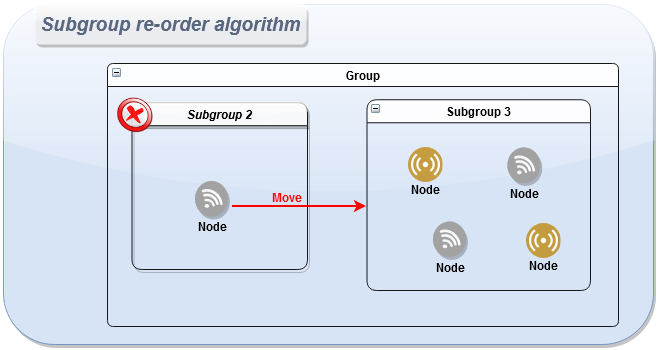
\includegraphics[scale=0.60]{figures/mgkmp/reorder.png}}
	\caption{MGKMP subgroup's re-order algorithm}
	\label{fig:re-order}
\end{figure}

A simple example to illustrate the kind of optimisation to bring on, is when a subgroup $S_1$ of cardinal $n=2$ is to merge with another subgroup $S_2$ of cardinal $n=8$, assuming we have a threshold $thr=2$. In this case, it would rather much more efficient to just assign the nodes from $S_1$ to $S_2$ and provide them with the necessary keys, instead of creating a new subgroup $S_3$. In this case, the 8 initial nodes from $S_2$ are saving all the computational power required for key generation as well as bandwidth for message exchanges for joining the of $S_3$. These 8 nodes have practically nothing to do. Moreover, the KM would have saved the computational energy for the creation of $S_3$, and its key generation.

\subsection{Sub-grouping sequences}
\label{subsec:subgroups}

As mentioned previously, layer 2 is intended for subgroup management. Nodes within a group are subdivided into multiple subgroups based on their minimal capabilities $mc$.This $mc$ value is determined through two main algorithms, referred as sequences: powers of two and Fibonacci.

\begin{figure}[htbp]
	\centerline{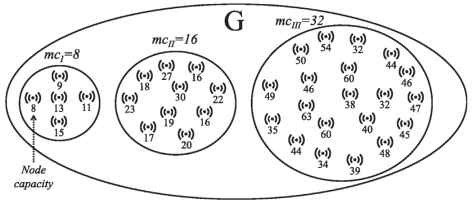
\includegraphics[scale=0.60]{figures/mgkmp/power2.png}}
	\caption{Source \cite{kandi_versatile_2020}: Example of a group partitioned using powers of 2 sequence}
	\label{fig:power2}
\end{figure}

This subgrouping sequences could be studied further, in order to eventually develop new efficient sequencing algorithms.

\section{Internal liabilities of MGKMP}
\label{sec:mgkmp_liabilities}

The corresponding working tracks seek to enhance the protocol’s security by looking into its performance when applied into practice. Many features of the protocol are demonstrated in a abstract and theoretical way. But some of the slightest behaviours in their concrete implementations might turn out to be extremely costy. Some of these features interact with each other, which can have implications on how they should be defined for practical implementation. The hereby considered problematic also deals with efficiency enhancement as well as security enforcement. So the point is to look out how practical the theoretical definitions of MGKMP are, and how to adjust eventual inconveniences.

\subsection{Refresh key generation}
\label{subsec:random_gen}

\begin{quote}{\emph{Robert R. Coveyou}}
	The generation of random numbers is too important
to be left to chance.
\end{quote}

%\begin{savequote}[45mm]
%	The generation of random numbers is too important
%to be left to chance.
%	\qauthor{Robert R. Coveyou}
%\end{savequote}

One of MGKMP's key properties is forward and backward. The main mechanism implemented to ensure it is the group rekeying process. As described in Section~\ref{sec:mgkmp_overview}, the new key is generated via a KDF which takes the old key and a random key $K_R$ as parameters. From a cryprographic point of view, the random generation is crucial to the whole process. Any vulnerability can blow the forward and backward secrecy up. An evicted or leaving node already has the old key. So if it gets hold of $K_R$, it can easily compute the new key. A recently joined node already has the new key. So if it gets hold of $K_R$, it will be possible to deduce the old one.

\begin{figure}[htbp]
	\centerline{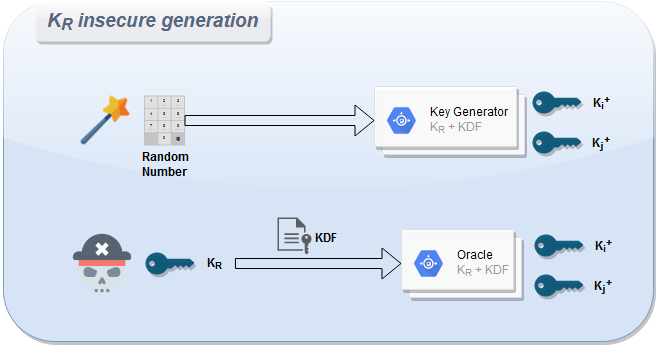
\includegraphics[scale=0.60]{figures/mgkmp/random.png}}
	\caption{Insecure $K_R$ generation}
	\label{fig:random_gen}
\end{figure}

Fig.~\ref{fig:random_gen} illustrates how an attacker who is able to guess $K_R$ and knows the KDF used, is able to compute newly generated secret keys by using some cryptographic oracle.

\subsection{Node's join authorization \& pre-secure channel}
\label{subsec:node_join}

The joining of a new node comes with two assumptions. First, the joining node is reliable and trustworthy. And the second implies that we dispose of a pre-existing secure channel between the Key Manager and and the joining node.
The first assumption don’t take into consideration the possibility that a node can already be compromised before it joining the network. Therefore, it burdens the risk of having all the new node’s keys systematically compromised.
The second assumption assumes the communication’s security between the Key Manager before having the node’s join process through. The non-compromising of all encryption keys related to the new node depends on this channel’s resilience.
In both cases above, we have a systematic key compromising situation just in the aftermath of a node’s join operation. This will eventually lead to have this node evicted afterwards, and hence, launching a rekeying upon leaving process.

\begin{figure}[htbp]
	\centerline{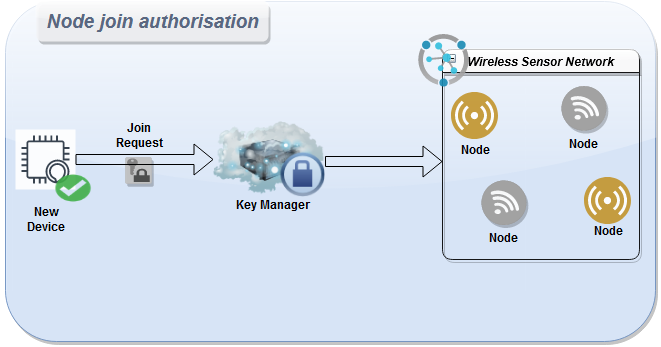
\includegraphics[scale=0.60]{figures/mgkmp/join_auth.png}}
	\caption{Node's join authorization}
	\label{fig:node_join}
\end{figure}

\subsection{Inadequate choice for cryptographic algorithms}
\label{subsec:cryptography}

Depending on the data to hash or encrypt, algorithms have to be considered with caution. It's easy to mistake cryptographic algorithms for an independant and irrelevant problem in our case. But MGKMP is protocol which directly deals with cryptography. When we look at common cryptographic issues, they are more related to the system implementation, rather than the algorithm itself. Although the algorithm's choice remains beyond the scope of this research work, it has to be thought in advance to facilitate the enginneer's work, who is actually implementing MGKMP. The point of this section is to underline the influence of protocol's design in hardening or easing the resilience of implemented cryptographic algorithms. It doesn't assume any lack or flaw in the protocol, such conclusion can only be the outcome of a dedicated study.

\subsubsection{Insecure key exchange}

Key exchange protocols solve a crucial problem, which is sharing a secret key between two communicating entities over an insecure channel. The most widely used protocol today is Diffie-Hellman. It can be implemented using discrete logarithms and elliptic curves. Even though the protocol is mathematically resilient, it's absolutely helpless against Man-in-the-Middle MITM attacks.

\subsubsection{Insecure hash functions}

Hash functions are very used in the MGKMP, but they have to be consiered carefully. Hash algorithms like MD5 or SHA-1 are utterly broken. SHA-2 hash family is more performant and safer than SHA-1, for its collision resistance. But once again, depending on the context, attacks like reduced-round collisions \cite{chowdhury_new_2008} or length extension attacks aren't excluded.

\subsubsection{Message authentication codes}

In relation with Section~\ref{subsec:node_join}, the use of Message Authentication Codes (MAC) is almost unavoidable. But that's a cryptographic challenge itself \cite{debian} and requires robust design of the related feature in MGKMP. For instance, prefix-MAC constructions is totally insecure even with SHA-2. Only SHA-3 algorithms allow the implementation of safe MAC systems.

\subsubsection{Signature algorithms}

The most robust signature algorithms available actually rely on public key cryptography. Attacks on RSA such as common modulus, hasted attack, Wiener's attack or common factor attack are leathal. How trustworthy asymmetric cryptography can be, it still has its own weaknesses. What is interesting is that these flaws aren't related to the crypto-system itself, but to its implementation. This means that these vulnerabilities should be carefully considered when designing a security system based on cryptography, as it's the case here.

\subsubsection{Lightweight cryptography algorithms}

Once more, the system designed here directly concerns cryptography. The resource-constraint nature of the IoT rather drives the attention towards lightweight cryptography algorithms \cite{bhardwaj_review_2017, surendran_survey_2018}. The choice of these algorithms has to take into account context requirements, since their characteristics differ according to the use case \cite{muthavhine_analysis_2018}. But something recurrent in these lightweight algorithms, is the curb of their resilience in favor of performance gain. This can be for example round reduction in AES algorithms, or the use of easy-to-generate initialization vectors (IV) in stream ciphers. If the host system (the MGKMP architecture in our case) allows it, such measures can lead to related-key attacks on AES \cite{hutchison_key_2010, hutchison_related-key_2009} or IV attacks on CBC and ECB.

\section{Analysis of the protocol's ecosystem}
\label{sec:ecosystem}

\begin{quote}{\emph{Pete Herzog --- The Open Source Cybersecurity Playbook}}
	The first key to any effective security game plan in knowing what you’re up against
\end{quote}

So far, the protocol’s related research work focused mainly on the conception the protocol’s processes and the exclusive definition of its internal core functionalities. In many cases, the development undertook a mathematical approach to identify different problems and solve them. However, the protocol shall be integrated in a probably complex environment, where its own functioning will influence and be influenced by external actors and components. This protocol already solve several critical security issues and significantly decrease the probability of an IoT network’s compromise. However, it’s only an actor in a bigger interconnected and hostile ecosystem.

This section seeks to provide some ideas for the analysis of these interactions, measurement of their impact on the well-functioning of the protocol, and suggestions to improve the protocol considering the conducted risk analysis. The point is to see the problematic from different angles in order to better apprehend the protocol’s ecosystem and the stakes which come along, in order to have a system practically compatible with any or at least most common environments seen in major use cases. Furthermore, some aspects of the protocol could be possibly enhanced in order to cover up for attack vectors coming from those actors and reduce the attack surface.

The previous threats and vulnerabilities enumeration demonstrate some of the possible attack vectors for cryptographic key compromising. Since our protocol aims mainly at securing cryptographic key exchange and encrypting data transmission, then these attack scenarios could of interest for study. In these examples, we demonstrate that an attacker does not necessarily have to break the protocol’s design itself in order to compromise the managed cryptographic keys. But he can however look for actors in the overall ecosystem interacting with our protocol, and take advantage of its eventual weaknesses.

The protocol’s environment to consider is pretty large and can include a variety of inter-connected actors interacting with our nodes and the Key Manager. Tiloca and Dini \cite{tiloca_grep_2016} already described an architecture in which the KM performs its duties. This architecture involves a Key Management System (KMS) operating above the KM. On the same level as the KMS, we have a Group Membership Service (GMS) keeping track of which nodes belong to the group. In our architecture, we can very intuitively imagine that this same service would also be keeping track of which nodes membership regarding subgroups as well. When a new node joins in or is evicted out of the group, the GMS should have a process to carry out in order update its membership lists. Still on the same level as the KMS, the architecture includes an Intrusion Detection Service (IDS), assuming the task of identifying malicious nodes and report them the GMS to have them evicted. Finally, on top of the three services (GMS, KMS and IDS), we have a group controller (GC), which role is to oversee the well functioning of these services. Fig.~\ref{fig:grep} illustrates the architecture described by the authors of the GREP protocol.

\begin{figure}[htbp]
	\centerline{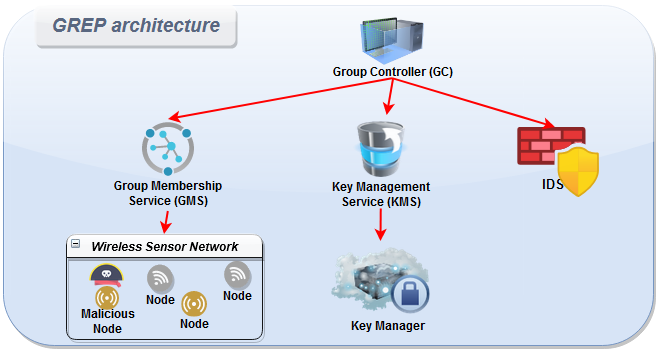
\includegraphics[scale=0.60]{figures/mgkmp/grep.png}}
	\caption{GREP architecture}
	\label{fig:grep}
\end{figure}

However, a realistic infrastructure in which the Key Management protocol shall be integrated is definitely much more sophisticated that the one described above. Fig.~\ref{fig:ecosystem} illustrates, in a non-exhaustive way, the diversity and complex interconnection of a realistic environment. We can see below the Key Manager and the Wireless Sensor Network which are embedded in the core of the protocol. But all around we have a dynamic and active ecosystem of several entities interacting with both. Among those entities, we have a firewall, through which go all transmissions from and to the group. There is as well the GMS and an IDS, as already discussed. In order to mitigate risks of a malicious node joining the group, we can imagine an Identity Access Management system in order to check out a node’s join request legitimacy. This IAM service can also assume other responsibilities in our environment. The IAM service, depending on the use case, can be substituted with an Access Control Server (ACS). As it’s more and more common, we can assume that our network is somehow related to some Cloud-based service. Therefore, additional security constraints are also to be considered by the protocol. Furthermore, the node’s architecture itself is an element worth attention, whether form a software or a hardware point of view. Further features such as logs generation by the KM for eventual forensics analysis can be considered too.

\begin{figure}[htbp]
	\centerline{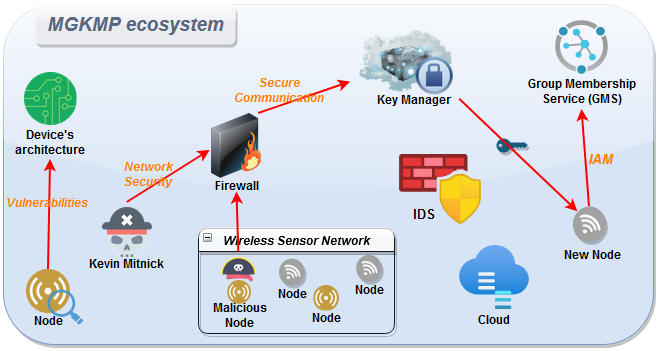
\includegraphics[scale=0.60]{figures/mgkmp/ecosystem.png}}
	\caption{Key Management protocol's ecosystem}
	\label{fig:ecosystem}
\end{figure}

From previous analysis, a number of attacks such as the low-level Sybil attack and RPL routing attacks are actually conducted by malicious nodes within the network. Our protocol doesn’t interfere in the detection process of veiled nodes. But it does make sure, throughout the rekeying upon leave process, that this node is indeed evicted and cannot access the network’s communications afterwards, ie. ensures forward secrecy.

Firewalls are a central element in IoT networks in order to filter out unnecessary or malicious network frames originally destined for some node, especially with the ever coming-back energy constraints. Yet, firewalls are also an attractive concentration point of network traffic. The compromise of the firewall, even partially through a foothold, might to the compromise of other nodes, if not the whole network. That’s why communications going through in and out should all be enough secured and authenticated, at risk of jeopardizing internal communications on the group. Among other reasons, this can significantly mitigate risks of insecure neighbor attacks. The device-to-device communications requires a prior steps of router discovery and address resolution. A firewall in the inside can make sure that these messages aren’t detoured to a malicious destination. The firewall can also be deployed to monitor these internal communications themselves, in which case node-to-node and KM-to-node messages will all go through the firewall. If the network’s security is not robust enough, a hacker would be able to eavesdrop on some communications allowing more damaging attacks such as fragmentation replay and duplication attack or just tampering with frames. The latter is actually a very serious threat as it opens the door for a bit-flipping attack.

The protocol is essentially designed to ensure cryptographic keys management and exchange between different nodes and the KM. As briefly explained above, the network’s infrastructure can sometimes be easily eavesdropped on. This ease in intercepting transmissions might very well allow an attacker to measure and analyse time required for nodes to perform protocol related encryption operation, exposing the protocol to a category of side-channel attacks, known as Timing attacks. This also intercross with the previously part mentioning the Timing attack.

In Section~\ref{subsec:node_join}, we discussed the problematic of the pre-established secure channel between the KM and new joining node. A reliable communication over this channel requires an end-to-end security on the transport layer. The purpose is to make ensure reception of a message by the desired destination while authenticating the sender. Here we go back to Message Authentication Codes (MAC) and message signature algorithms, already discussed in Section~\ref{subsec:cryptography}. This measure concerns joining nodes as well as device-to-device communications. Device-to-device communications should also bare the network security aspect since they are subject to session establishment and resumption attacks. These attacks can badly affect the integrity of, among others, some Data Encryption Keys (DEKs).

To quickly sum up the previous, we have a recurring problem, which is node compromising. It’s here where the importance of malicious node detection stands out. For this point, we already assumed the likely presence of an IDS in our ecosystem. We have also considered a firewall filtering internal communications of the group, in which case it can also monitor the network traffic in the same time to detect abnormal behaviours. An independent monitoring solution, such as a Zabbix server, could be considered too, while its output can be used for veiled activities detection. Depending on which solution is to be used, we need to make sure that different operations carried out by the Key Management will always be compatible with its environment. We can even consider different versions of the protocol for each use case, with eventual optimisations for each facilitating the bad nodes hunt. All of this requires a standalone study and analysis to select what can possibly be done on this path.

Besides, all previously mentioned entities such as IAM service, firewalls and ACS are actively interacting with the group nodes and the KM, as already mentioned. To some extent, and depending on the situation, some on them could even be considered as insider actors of the group communication. Hence, they are technically members of the group, requiring encryption keys provided by the KM on their turn. As a consequence, an other study and analysis could be carried out to precise (i) which keys exactly these elements will need to efficiently assume their functions, (ii) how are they going to be distributed by the KM and also regarding the other nodes, and foremost (iii) how the KM should handle them and manage their keys. This study shall improve the implementability of the protocol and make it easier to integrate in a concrete industrial application.

Finally, the Key Management protocol already takes into consideration different characteristics of IoT devices, such as their low computation power or constrained energy capacity. Those considered characteristics are mainly physical though. There is much more in the devices to be studied in order to analyse its implication of well functioning of the protocol. In case of popping up issues, optimisations and improvement shall be made on the protocol’s design to make it further operational. This study turns around the devices systems, from the hardware as well as the software point of view.

On the software level, we have already mentioned some typical threats including malwares. A malware-infected node can easily have all its stored encryption keys compromised. To this purpose, we can think of some security mechanisms regarding how keys are to be stored on the device. These mechanisms have already been thought in the protocol, but only regarding the storage overhead. So a further study of this part can very well enhance the integrity of the protocol.
From the hardware point of view, two main elements should be considered to assess the protocol’s efficiency and usability in its environment: (i) the device’s firmware and (ii) the processor’s architecture. The hardware study is crucial as it allows the assessment of the risk level regarding a possible rootkit compromising. Same as for malwares, a rootkit infected node can easily have all of  its encryption keys compromised. Nevertheless, rootkits are far more lethal than high level malwares and foremost, they are extremely stealthy and hard to detect, if they are detectable. Rootkits raise the interest of studying the processor’s architecture besides the firmware. The interest in considering processors architectures could come from other threats too, like the Timing attack. An analysis can conclude on whether the protocol’s key exchange and storage processes take this kind of threat into account or not, then conclude on which enhancements, if possible, can be added to make the protocol more resilient.